\section{实验部分 - UCB}

\subsection{基本结构}

实验主要分为三个主要的python文件

\begin{itemize}
    \item UCB.py: 主程序,负责调用其他模块
    \item utils.py: 工具函数,负责处理数据和模型
    \item visualization.py: 可视化函数,负责可视化结果
\end{itemize}

接下来依次介绍每个文件的实现思路

\subsection{utils.py}

\subsubsection{估值函数}

首先需要为玩家生成估值函数,其数学表达式为

\[
   v(n) = C * (1 - e^{-\beta * n})
\]

其中,$C$ 是估值函数的最大值,$\beta$ 是估值函数的衰减系数。

这个函数当$n$趋近于无穷大时,$v(n)$趋近于$C$,当$n=0$时,$v(n)=0$。

而且满足$v(n)$随$n$的增大而增大,并且增速越来越小,边际收益递减。

然后根据玩家的类型,生成不同参数的估值函数,用于模拟不同玩家的行为。

具体来说通过base\_rate和max\_value两个参数来控制估值函数的形状。

\subsubsection{生成价格曲线集合}

根据论文中的算法2,生成一个离散化的价格曲线集合,而且是$m-step$的,即跳跃次数不超过$m$次。

算法2的实现主要分为三个步骤:

\paragraph{步骤1:构建数据空间网格 $N_D$}

首先构建数据空间网格,用于离散化数据点数量$n$:

\begin{itemize}
    \item 设定阈值 $threshold\_n = \lfloor \frac{2Jm}{\epsilon^2} \rfloor$
    \item 对于 $n \leq threshold\_n$ 的数据点,不进行离散化,直接添加到网格中
    \item 对于 $n > threshold\_n$ 的数据点,采用对数离散化:
    \begin{itemize}
        \item 计算 $Y_i$ 点:$Y_0 = threshold\_n$,$Y_{i+1} = Y_i \cdot (1 + \epsilon^2)$
        \item 在相邻的 $Y_i$ 点之间插入约 $2Jm$ 个内点
        \item 使用线性插值生成内点:$inner\_points = linspace(Y_i, Y_{i+1}, 2Jm)$
    \end{itemize}
    \item 最终将0也加入网格中,确保包含不购买的情况
\end{itemize}

\paragraph{步骤2:构建估值空间网格 $W$}

然后构建估值空间网格,用于离散化价格水平:

\begin{itemize}
    \item 计算 $Z_i$ 点:$Z_0 = \epsilon$,$Z_{i+1} = Z_i \cdot (1 + \epsilon)$
    \item 在相邻的 $Z_i$ 点之间进行细粒度插值:
    \begin{itemize}
        \item 计算间隔:$gap = Z_i \cdot \frac{\epsilon}{m}$
        \item 计算插值步数:$num\_steps = \lfloor \frac{Z_{i+1} - Z_i}{gap} \rfloor$
        \item 使用线性插值生成内点:$inner\_points = linspace(Z_i, Z_{i+1}, num\_steps)$
    \end{itemize}
    \item 最终将0也加入网格中,确保包含免费价格
\end{itemize}

\paragraph{步骤3:生成m-阶梯价格曲线}

基于上述两个网格,随机采样生成m-阶梯价格曲线:

\begin{itemize}
    \item 首先添加一条"免费"价格曲线(全零价格),这是算法3第一轮必需的
    \item 对于每条新的价格曲线:
    \begin{itemize}
        \item 随机决定阶梯数 $k \in [1, m]$
        \item 从 $N_D$ 中随机选择 $k$ 个跳变点 $jump\_points\_n$
        \item 从 $W$ 中随机选择 $k$ 个价格水平 $price\_levels$
        \item 构建阶梯价格曲线:
        \begin{align*}
            p(n) = \begin{cases}
                price\_levels[0] & \text{if } 0 \leq n \leq jump\_points\_n[0] \\
                price\_levels[1] & \text{if } jump\_points\_n[0] < n \leq jump\_points\_n[1] \\
                \vdots \\
                price\_levels[k-1] & \text{if } jump\_points\_n[k-2] < n \leq jump\_points\_n[k-1] \\
                price\_levels[k-1] & \text{if } n > jump\_points\_n[k-1]
            \end{cases}
        \end{align*}
    \end{itemize}
\end{itemize}

这种离散化方法确保了价格曲线集合的大小是多项式级别的,同时保持了足够的表达能力来近似最优解。




\subsubsection{生成估值函数集合}

在UCB算法中,需要预先计算每个(价格曲线, 买家类型)组合的购买决策和收入,这模拟了Agent拥有的先验知识。

\paragraph{购买决策计算}

对于每个价格曲线$p$和买家类型$i$,计算最优购买量:

\begin{itemize}
    \item 计算所有可能购买量$n$的效用:$u_i(n) = v_i(n) - p(n)$
    \item 找到效用最大化的购买量:$n^* = \arg\max_{n} u_i(n)$
    \item 如果最大效用小于0,则选择不购买($n^* = 0$)
    \item 如果存在多个效用相等的最大值,根据论文规则选择最大的$n$
\end{itemize}

\paragraph{收入计算}

基于购买决策计算收入:

\begin{itemize}
    \item 收入矩阵:$revenues[i,j] = p_j(n^*_{i,j})$,其中$p_j$是第$j$条价格曲线,$n^*_{i,j}$是类型$i$买家在价格曲线$j$下的最优购买量
    \item 购买量矩阵:$purchases[i,j] = n^*_{i,j}$,记录每种组合的购买量
\end{itemize}

这种预计算方式确保了算法在运行时能够快速查询任何价格曲线和买家类型组合的预期收入,为UCB算法的决策提供基础数据。

\subsection{UCB.py}

\subsubsection{Config}

配置类负责管理实验参数和生成真实的买家类型分布:

\begin{itemize}
    \item \textbf{基本参数}:
    \begin{itemize}
        \item $M\_TYPES$:买家类型数量(默认10)
        \item $N\_ITEMS$:数据点总数(默认100)
        \item $T\_HORIZON$:总回合数(默认$M\_TYPES \times 10000$)
        \item $J$:收益递减常数(默认2.0)
        \item $\epsilon$:近似精度参数(默认0.1)
        \item $num\_samples$:生成的价格曲线数量(默认$\max(7, M\_TYPES + 5)$)
    \end{itemize}
    \item \textbf{真实分布生成}:根据买家类型数量自动生成合理的概率分布
    \begin{itemize}
        \item 对于1-4种类型,使用预设的分布
        \item 对于更多类型,使用高斯分布生成后归一化
    \end{itemize}
\end{itemize}

\subsubsection{UCBAgent}

实现了论文中算法3的UCB算法,主要包含以下函数:

\paragraph{初始化}

\begin{itemize}
    \item 初始化内部状态:$t = 1$(当前回合数)
    \item $T_i$:类型$i$被"探索"的次数
    \item $N_i$:类型$i$被实际观察到的次数
    \item 历史记录字典:用于存储学习过程数据
\end{itemize}

\paragraph{choose\_action}

根据UCB规则选择价格曲线:

\begin{enumerate}
    \item 第一轮强制选择免费价格曲线(索引0)
    \item 计算经验估计:$\bar{q}_i = \frac{N_i}{T_i}$
    \item 计算置信度奖励:$\sqrt{\frac{\log T}{T_i}}$
    \item 构造乐观估计:$\hat{q}_i = \bar{q}_i + \sqrt{\frac{\log T}{T_i}}$
    \item 计算UCB收入:$\hat{rev}(p) = \sum_{i=1}^m \hat{q}_i \cdot revenue(p, i)$
    \item 选择UCB收入最高的价格曲线
\end{enumerate}

\paragraph{update}

根据环境反馈更新内部状态:

\begin{itemize}
    \item 更新探索次数:$T_i \leftarrow T_i + 1$(对于所有会购买类型$i$的买家)
    \item 更新观察次数:$N_i \leftarrow N_i + 1$(如果本轮观察到类型$i$买家)
    \item 记录历史数据:回合数、动作、收入、买家类型等
\end{itemize}

\subsection{visualization.py}

最后根据记录到的历史数据,绘制出UCB算法的可视化表现,代码不再赘述,接下来展示结果


\subsection{实验结果}

\begin{figure}[H]
    \centering
    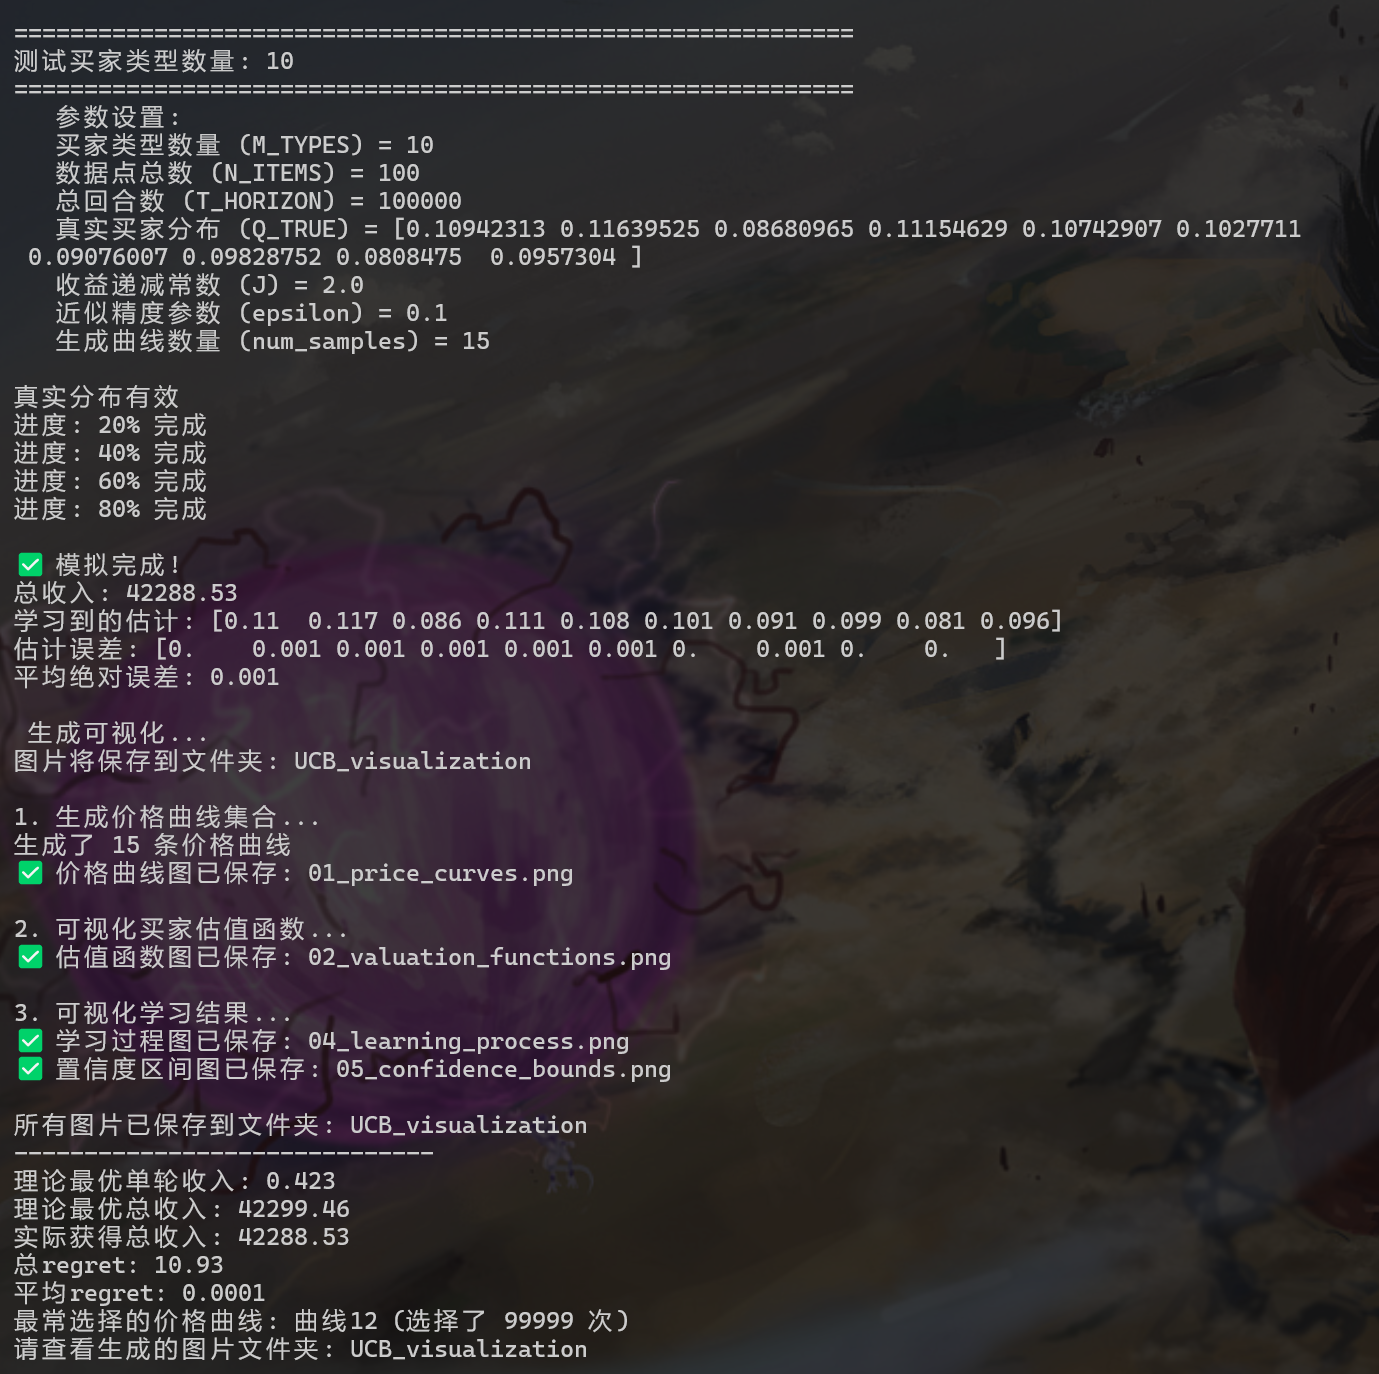
\includegraphics[width=0.7\textwidth]{figures/UCB1.png}
    \caption{UCB算法结果}
\end{figure}

可以看到,学习到的估计和真实分布非常接近,说明UCB算法能够很好地学习到真实分布。

\begin{figure}[H]
    \centering
    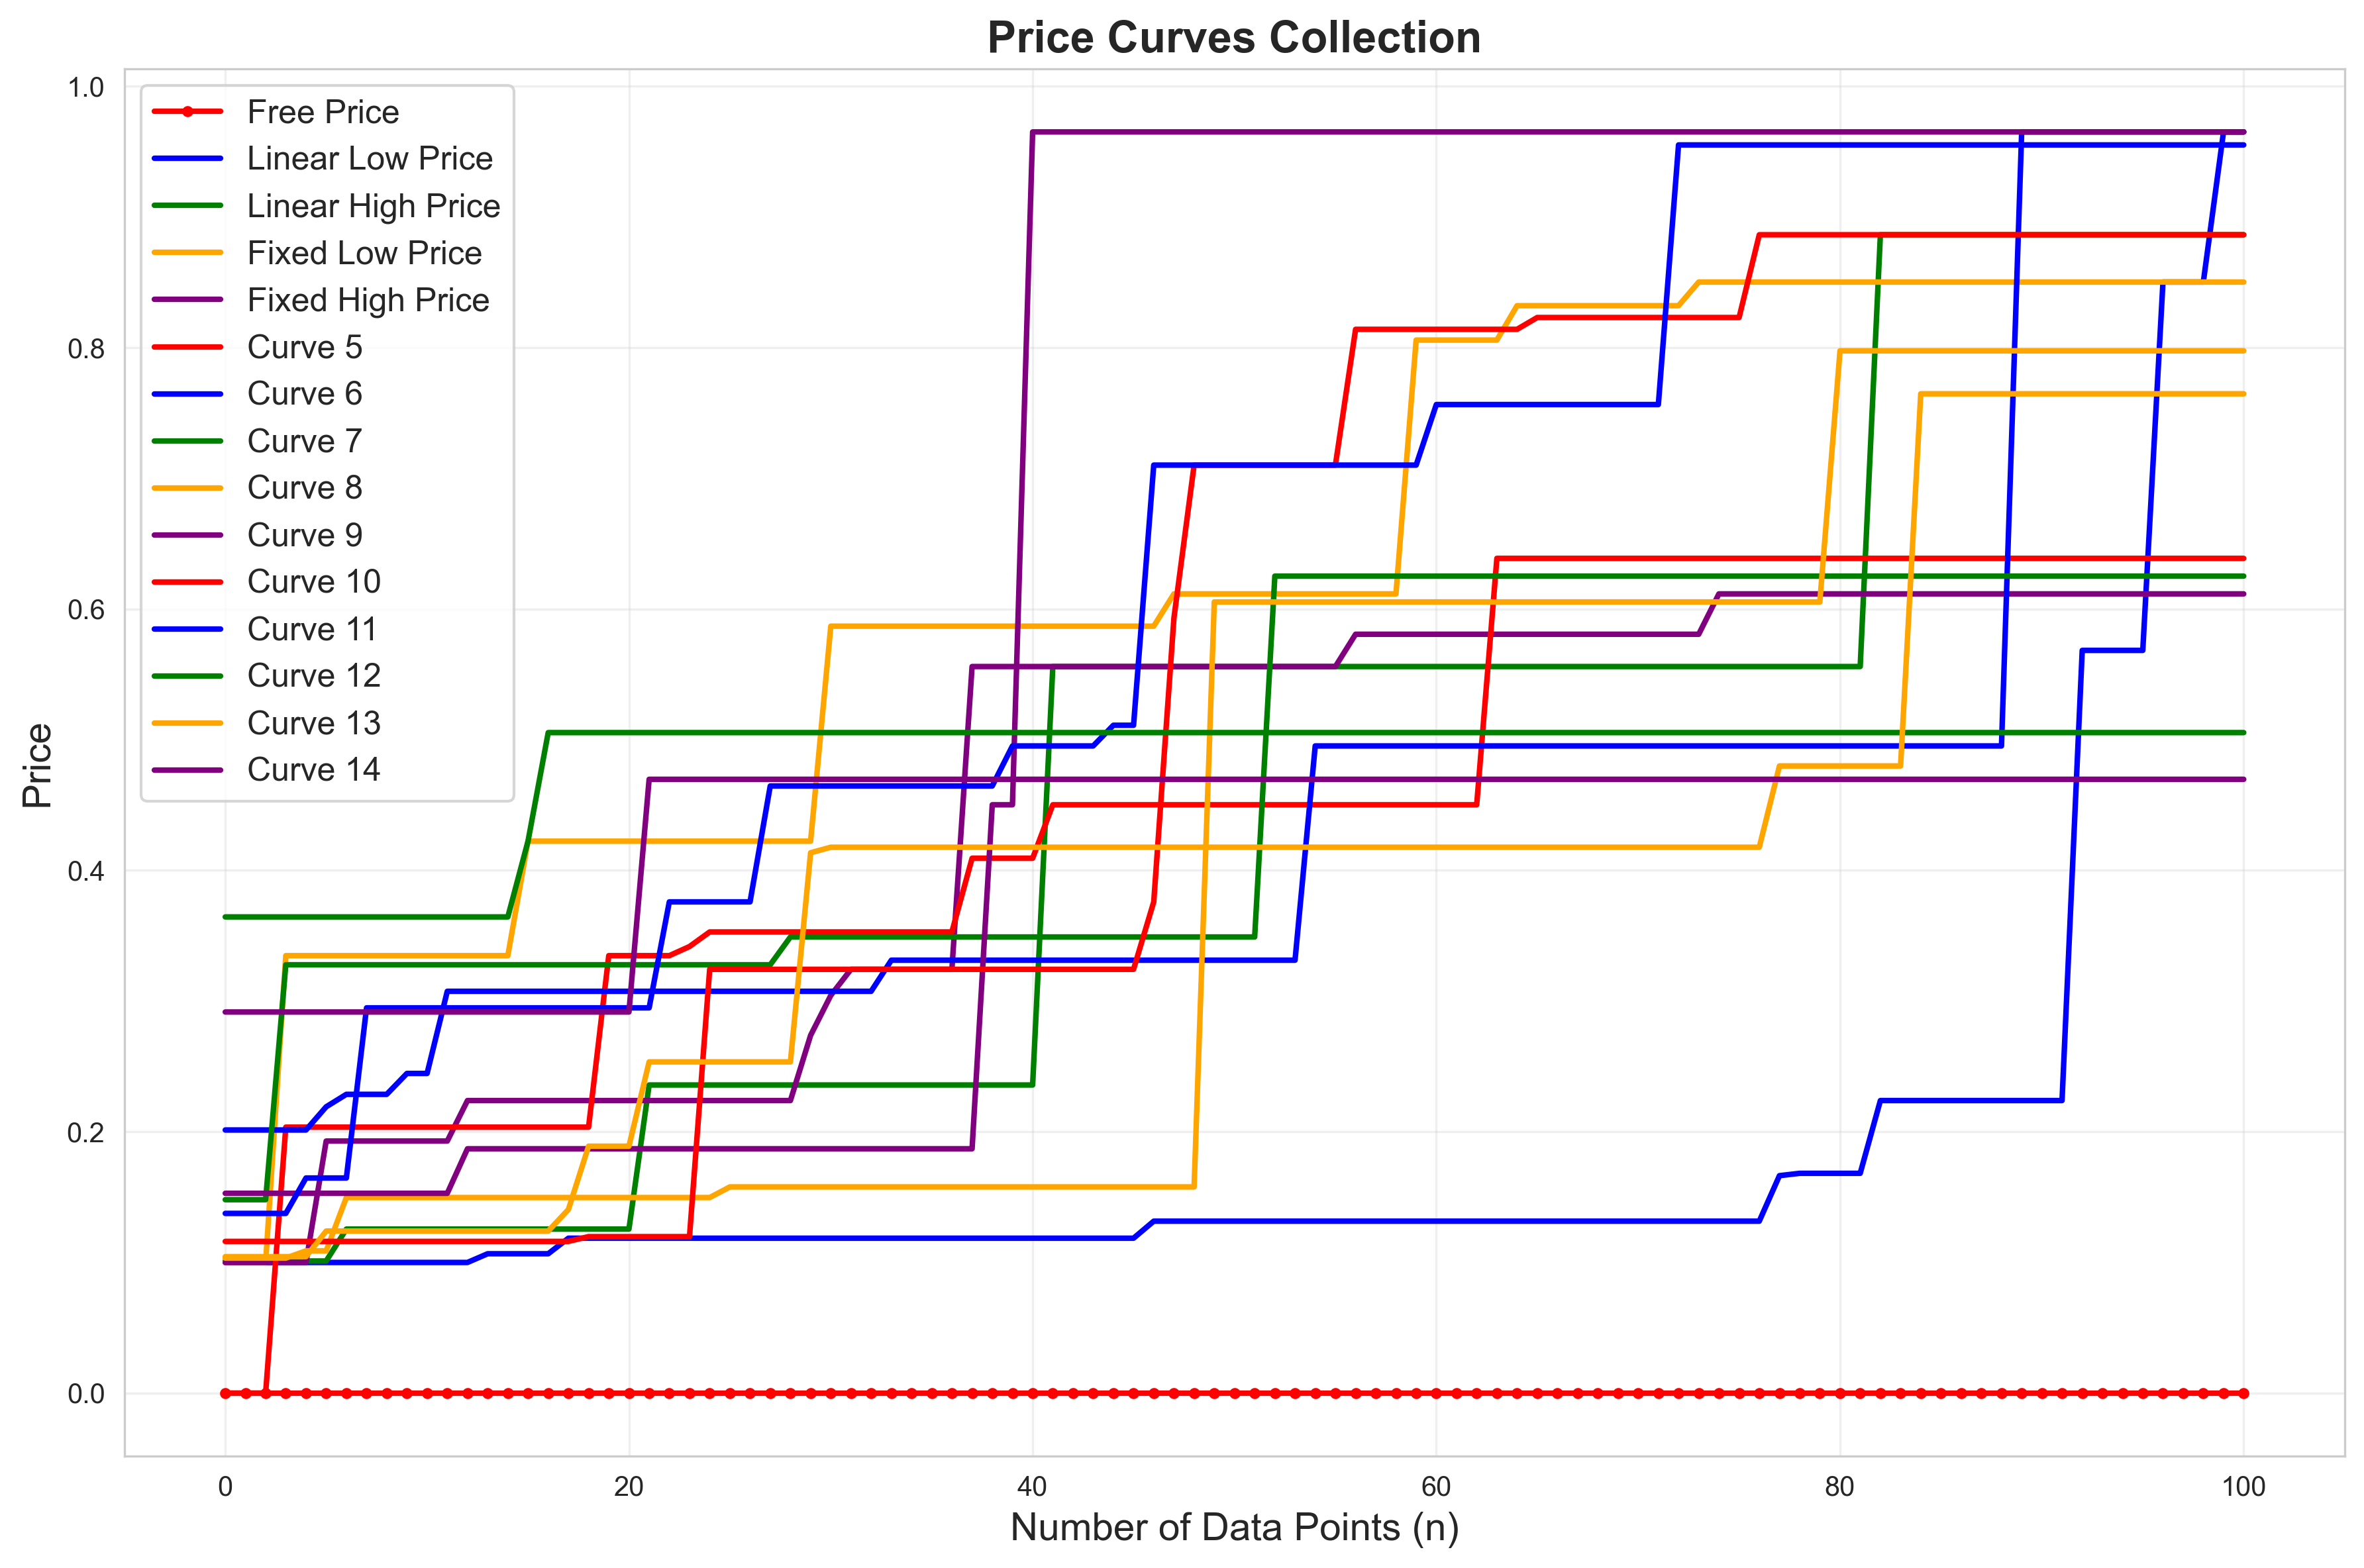
\includegraphics[width=0.7\textwidth]{figures/01_price_curves.png}
    \caption{价格曲线}
\end{figure}

可以看到价格曲线确实是阶梯状的,符合论文中的描述。

\begin{figure}[H]
    \centering
    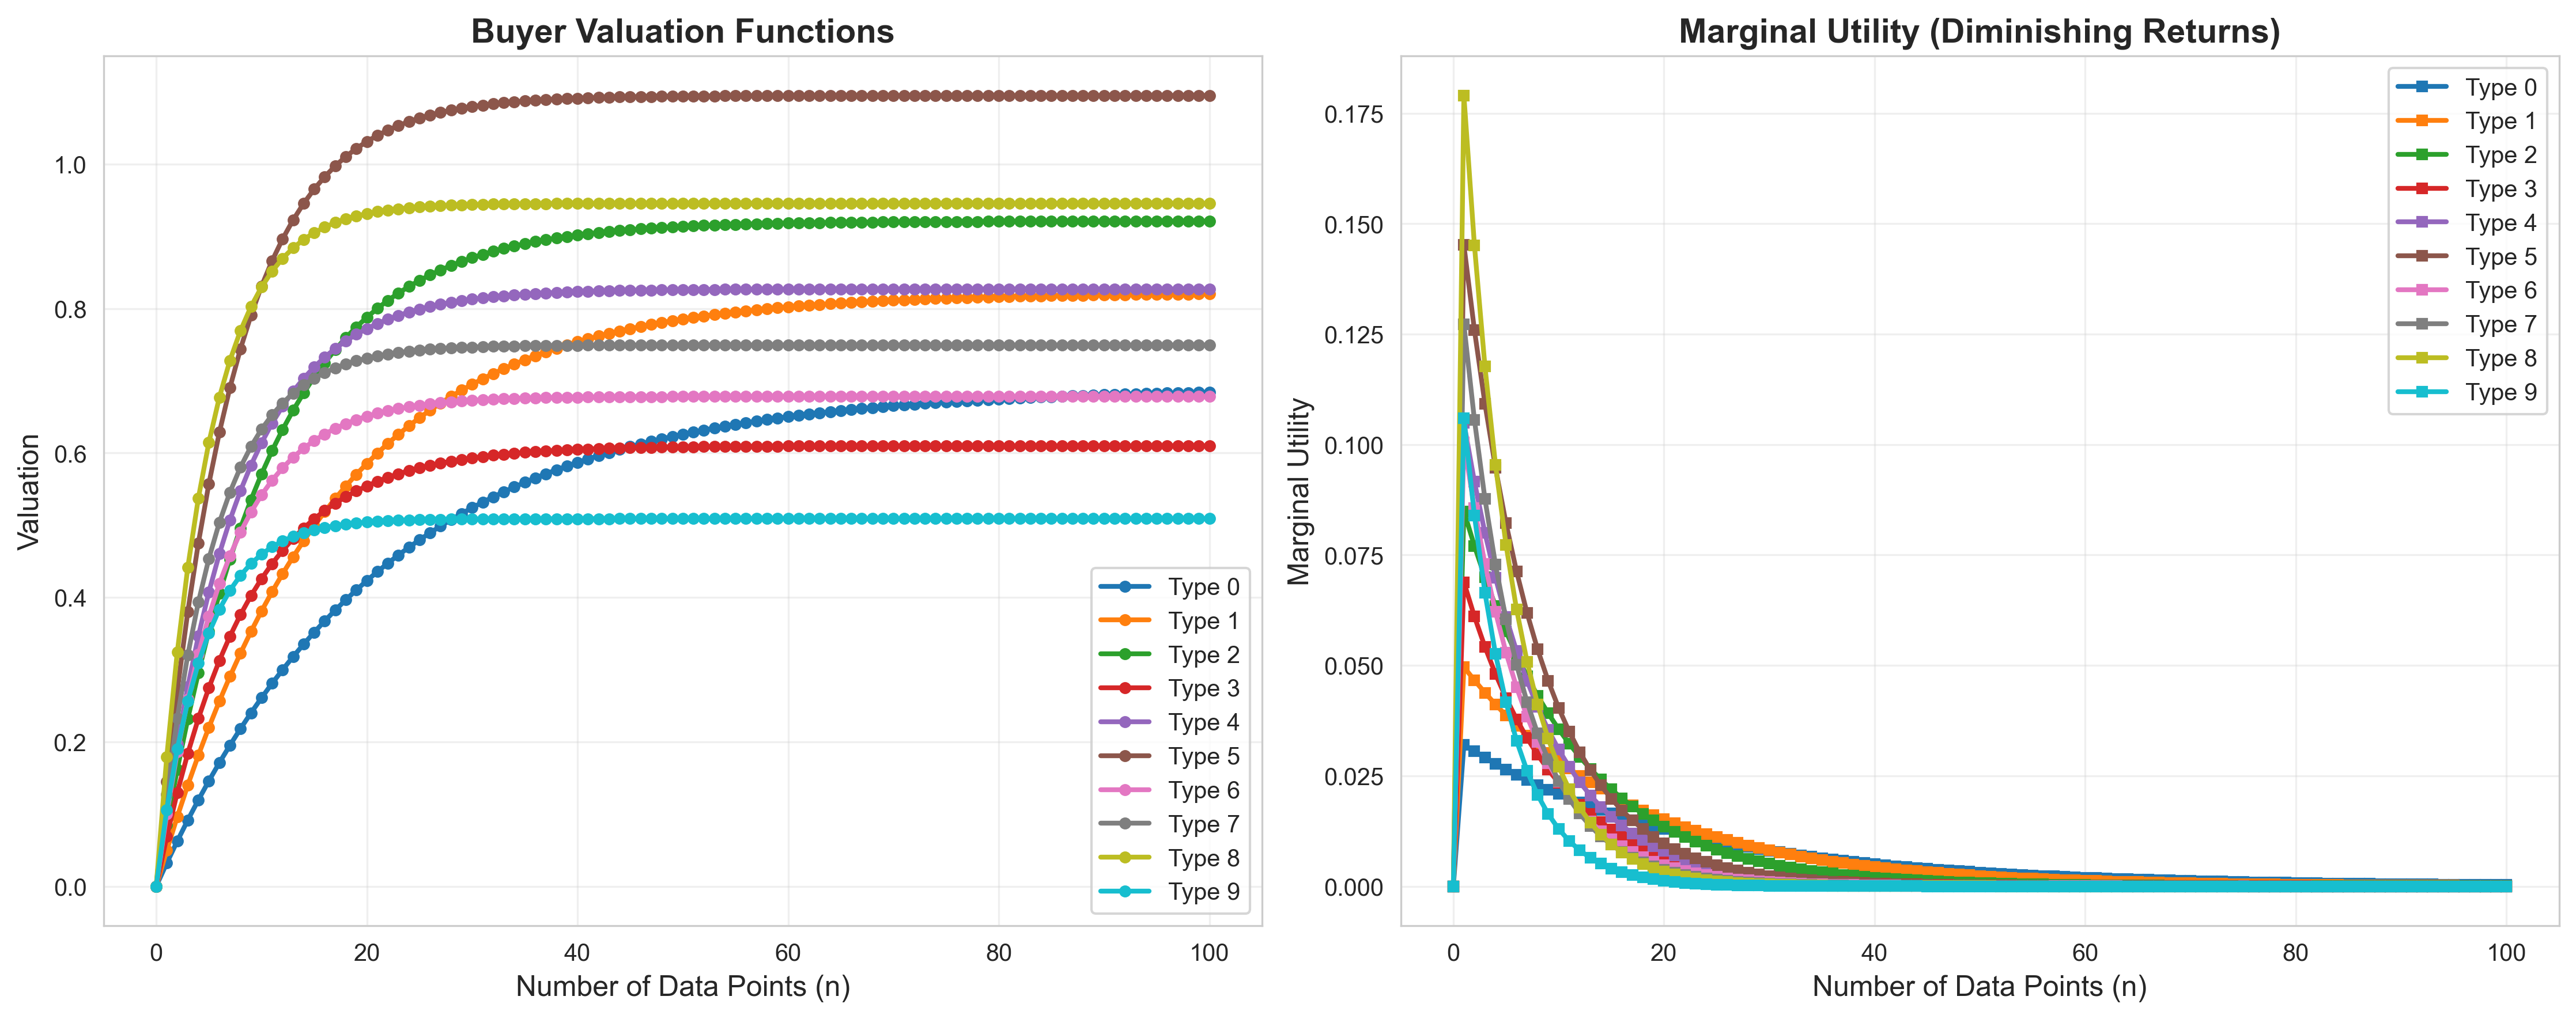
\includegraphics[width=0.7\textwidth]{figures/02_valuation_functions.png}
    \caption{估值函数}
\end{figure}

估值函数也与满足我们的要求

\begin{figure}[H]
    \centering
    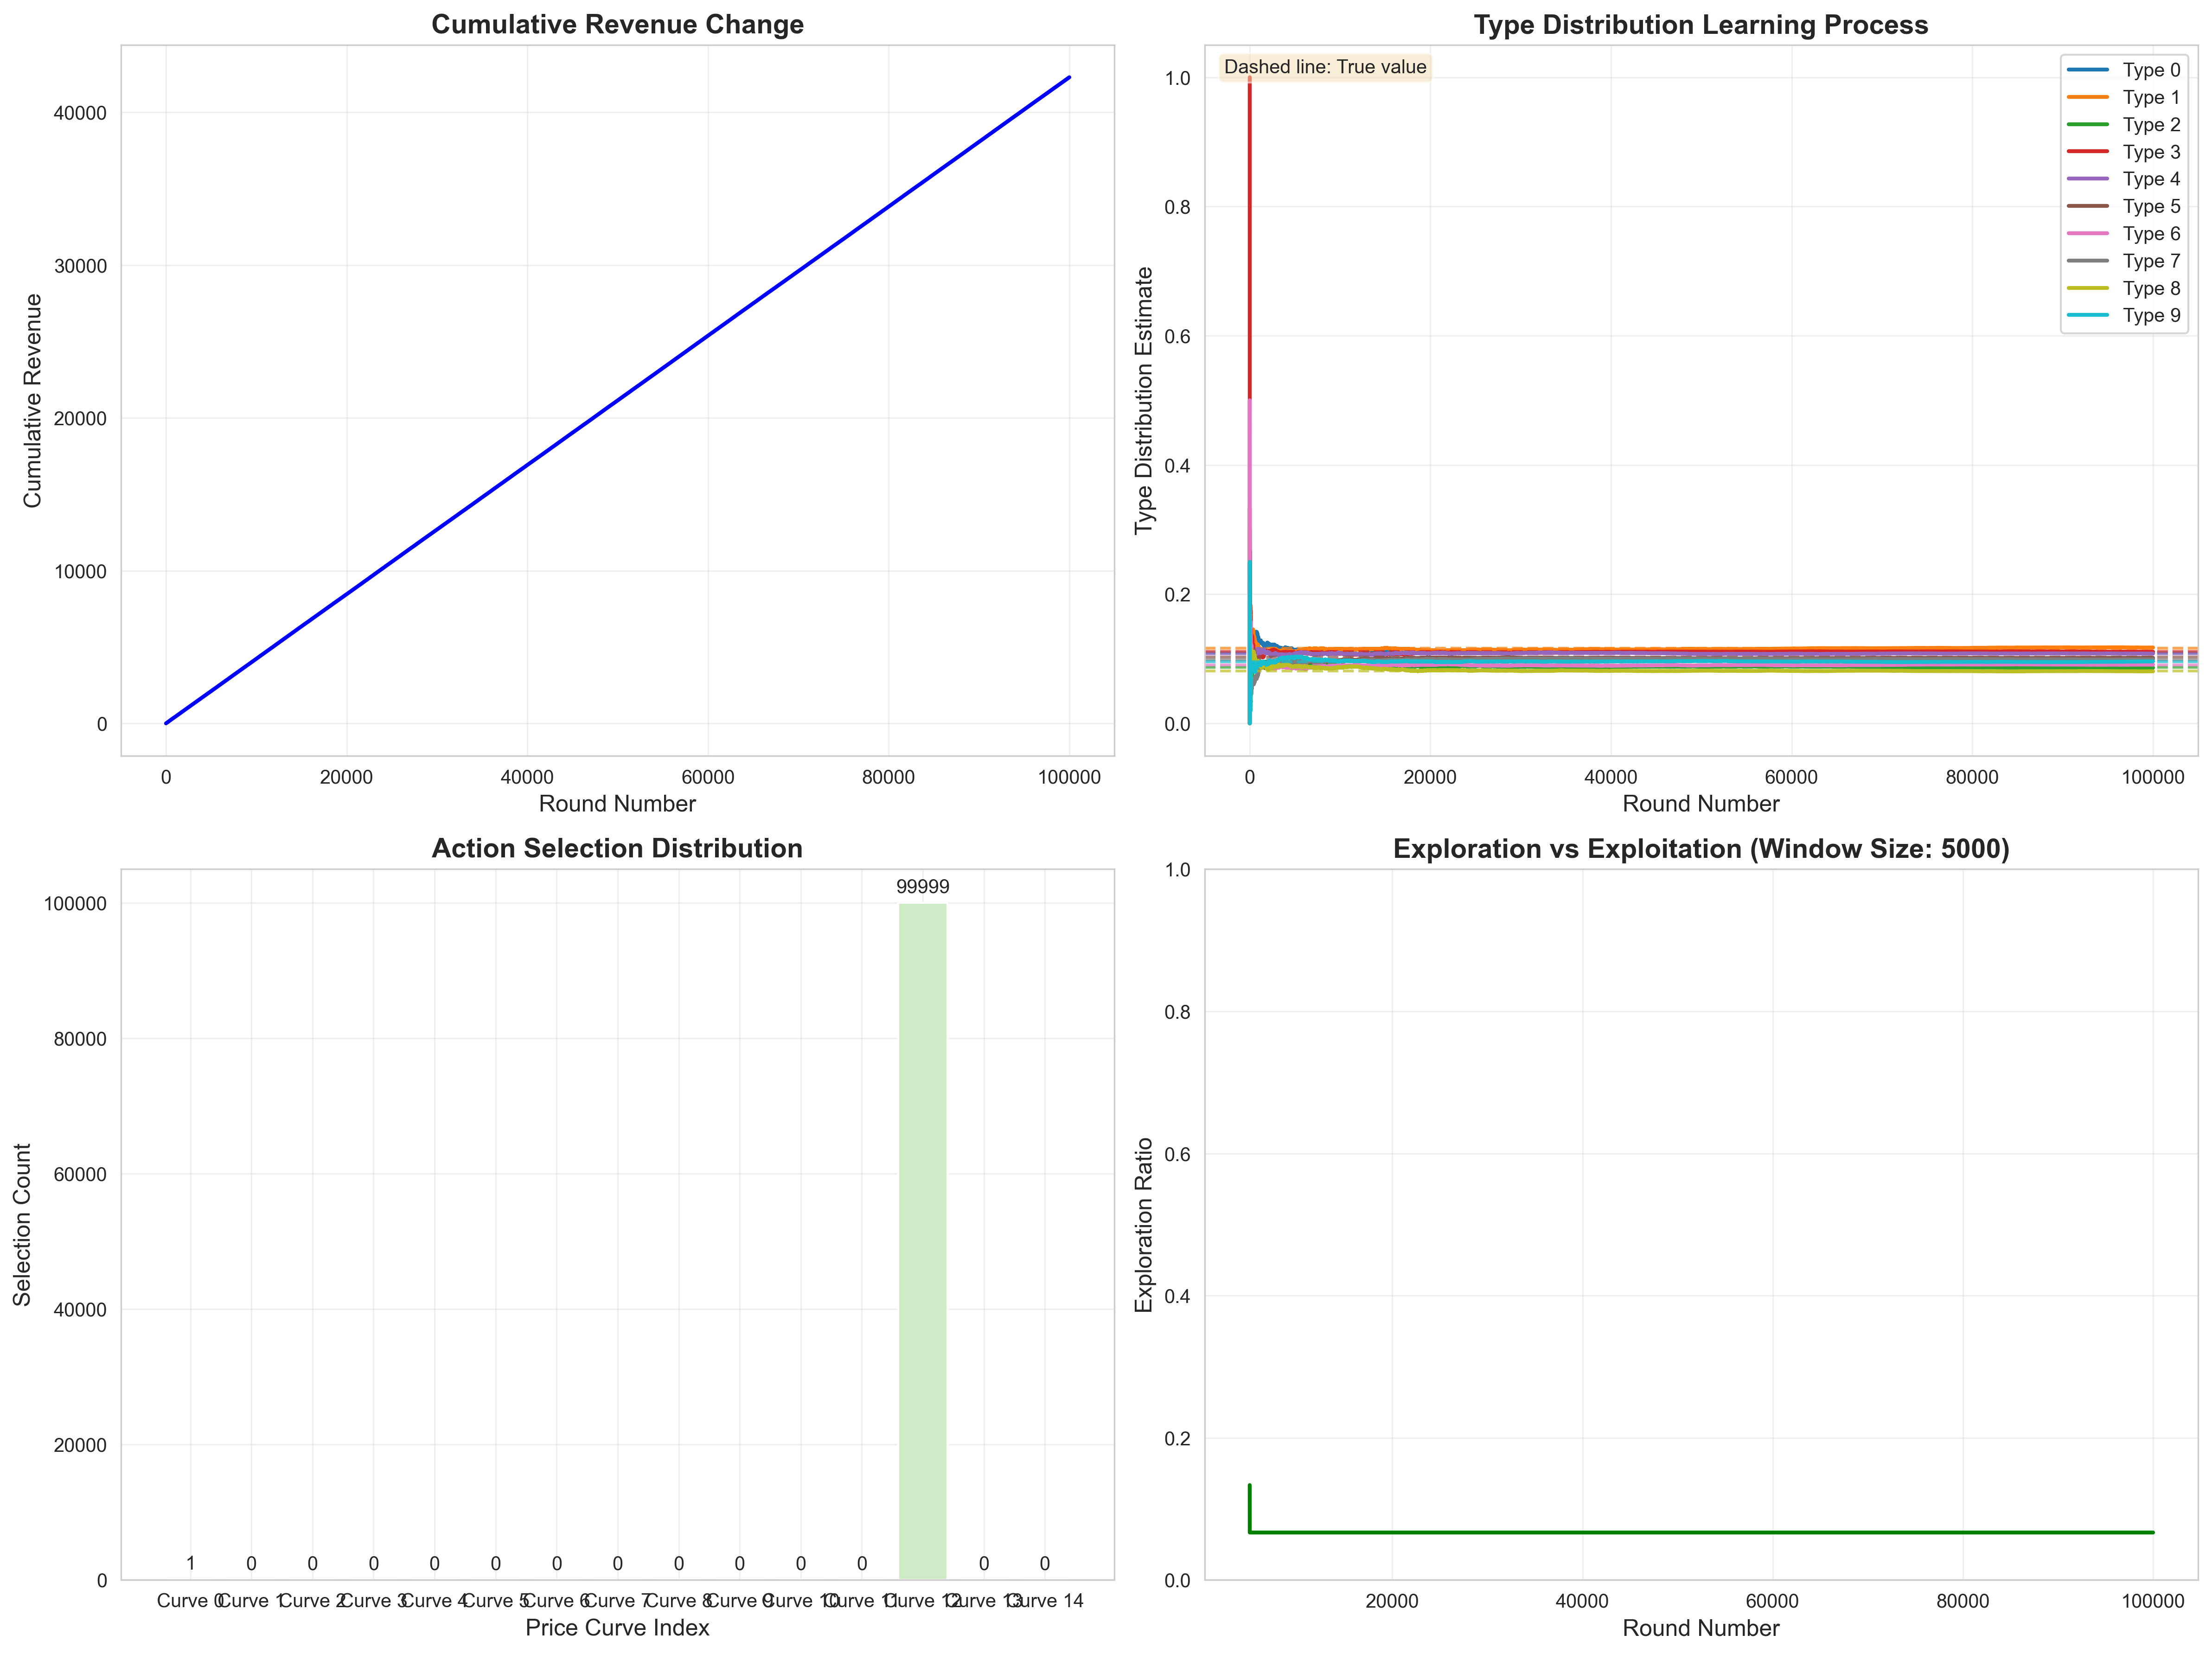
\includegraphics[width=0.8\textwidth]{figures/04_learning_process.png}
    \caption{学习过程}
\end{figure}

\begin{figure}[H]
    \centering
    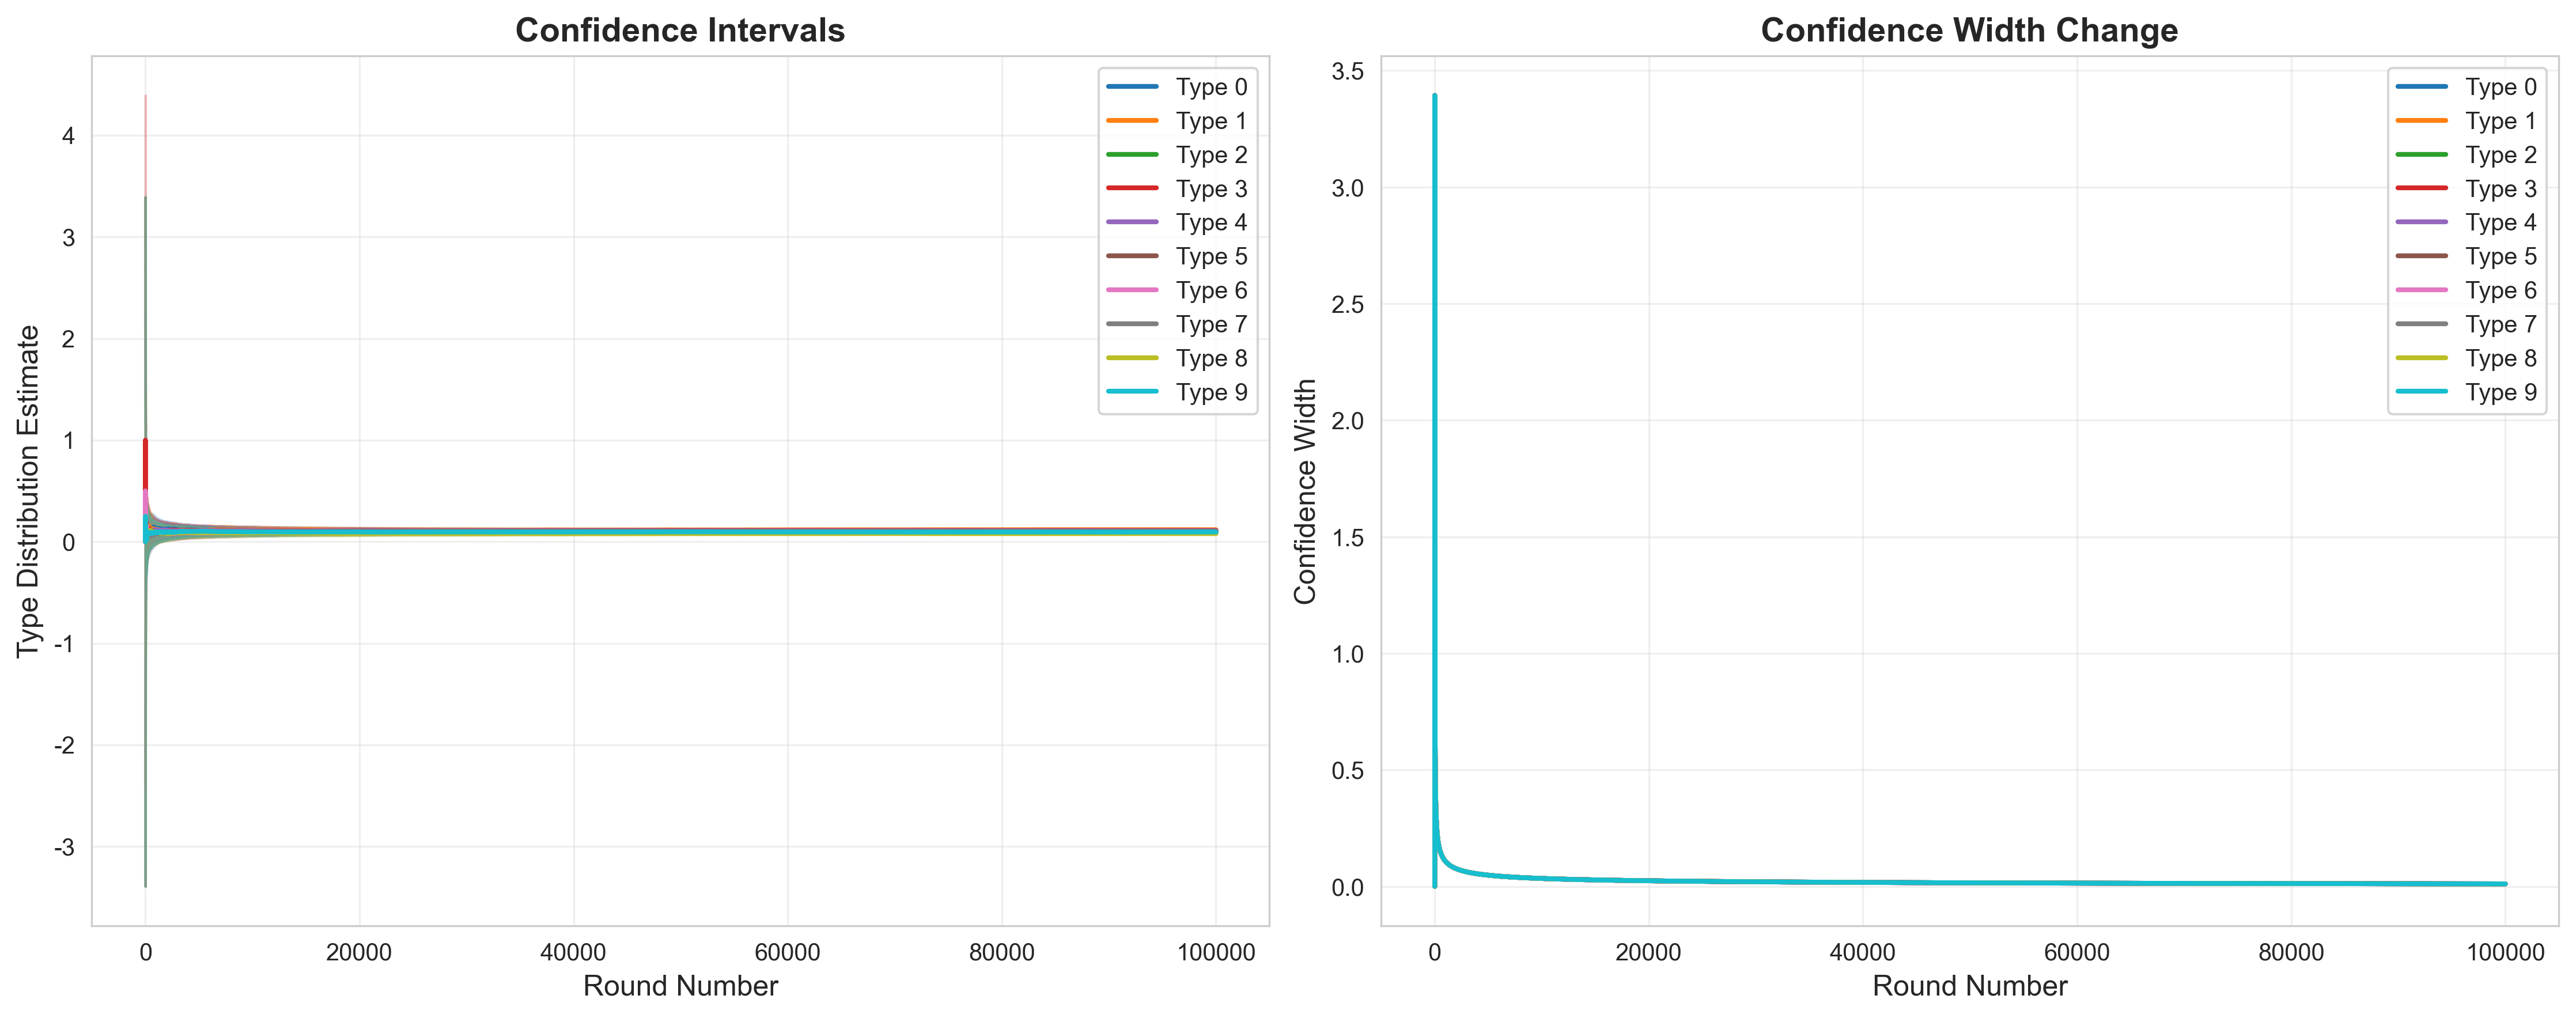
\includegraphics[width=0.8\textwidth]{figures/05_confidence_bounds.png}
    \caption{UCB 置信界}
\end{figure}

随着回合数的增加,置信界逐渐缩小,也满足我们的预期;








